%Nama Kelompok: Hardware
%Kelas: D4 1B
%Alit Fajar 1174057
%Berlian 1174034
%Ichsan 1174058
%Kevin 1174059
%Iqbal Hambali 1174060
%Virga 1174065

\section{Definisi}
Perangkat keras komputer adalah komponen fisik atau komponen komputer, seperti monitor, keyboard, penyimpanan data komputer, kartu grafis, kartu suara dan motherboard. Sebaliknya, perangkat lunak adalah instruksi yang bisa disimpan dan dijalankan oleh perangkat keras.
Perangkat keras diarahkan oleh perangkat lunak untuk menjalankan perintah atau instruksi apapun. Kombinasi perangkat keras dan perangkat lunak membentuk sistem komputasi yang dapat digunakan
Hardware atau yang kita kenal sebagai perangkat keras adalah suatu perangkat dalam komputer yang dapat dilihat secara langsung maupun dapat
disentuh, perangkat keras ini dapat mendukung berjalannya suatu komputerisasi. Perankat keras dapat bekerja apabila ada perintah yang
dilakukan kepada perangkat keras ini. Secara fisik, perangkat keras memiliki komponen-komponen yang terdiri dari suatu sistem. Sistem
adalah suatu komponen-komponen yang saling berhubungan dan saling mendukung. Jika salah satu komponen tidak berfungsi, maka proses-
proses dalam komputer tidak berjalan dengan baik.

\subsection{Sejarah Hardware}
Hardware atau dalam bahasa Indonesianya perangkat keras pertama kali dikemukakan oleh seorang ilmuan matematik ternama yang berkewarga
kenegaraan Inggris. Namanya Charles Babbage, beliau menciptakan suatu mesin hitung yang disebut difference engine pada tahun 1822.
Belum puas dengan penemuannya tersebut Charles Babbage memulai pengembangan penemuan sebelumnya yaitu difference engine menjadi
analytical engine yang dapat melaksanakan kalkulasi apa saja. Pada tahun 1833 analytical engine pun berhasil Charles Babbage temukan
dan mesin ini dikenal sebagai mesin General Purpose Digital Computer. Charles Babbage pun dikenal sebagai bapak komputer modern.

Belum selesai dari itu pada tahun 1937 seorang profesor ahli matematika dari universitas terkenal Havard Prof. Howad Aikem merancang
pembuatan sebuah komputer yag mampu melakukan operasi aritmatika dan logika secara otomatis. Setelah itu Prof. Howad Aikem memulai
kerjasamanya dengan perusahan IBM pada tahun 1944 untuk menyelesaikan komputer secara elektronik dan dinaminya \"Havard MARK I\" atau
Automatic Sequence Controlle Calculator (ASCC).

Sejarah perkembangan Hardware dapat dibedakan dalam 2 periode yaitu periode sebelum tahun 1940 dan periode sesudah tahun 1940. 
sebelum tahun 1940 dapat dikatakan sebagai evolusi komputer dengan teknologi mekanik. sejarahnya komputer dimulai ketika lahirnya 
komputer generasi yang pertama dengan nama Electronic Numerical Integrator and Calculator atau yang lebih banyak dikenal orang dengan 
nama computer ENIAC, padahal komputer digital pertama sebenarnya adalah Atanasoff-BErry computer atau disingkat dengan ABC,
pendirinya yaitu bernama Vincent Atanasoff.
 
\subsection{Generasi Pertama Perangkat Keras}
sejarahnya komputer dimulai ketika lahirnya 
komputer generasi yang pertama dengan nama Electronic Numerical Integrator and Calculator atau yang lebih banyak dikenal orang dengan 
nama computer ENIAC, padahal komputer digital pertama sebenarnya adalah Atanasoff-BErry computer atau disingkat dengan ABC,
pendirinya yaitu bernama Vincent Atanasoff. Pada generasi yang pertama Dr. John W Mauchly dan rekannya J. Presper Eckert membuat 
komputer yang disebut ENIAC. Electronic Numerical Integrator and Calculator atau ENIAC dibuat 1942, yang tujuan pembuatannya untuk
membantu Amerika Serikat menghitung target sasaran bom pada perang dunia kedua, Electronic Numerical Integrator and Calculator atau 
ENIAC sebenarnya lebih dikenal dengan sebutan Vacum Tube.

\subsection{Genereasi Kedua Perangkat Keras}
Era Vacum Tube sudah mulai tergantikan oleh generasi kedua ini. Pada tahun 1959 Transistor menggantikan Vacum Tube dalam
menyimpan dan melakukan proses informasi. Dikarenakan Transistor memilik bentuk yang lebih kecil dari Vacum Tube, dan juga lebih tenang
dikarenakan tidak mudah panas, serta tidak begitu banyak energi yang dibutuhkan untuk menjalankannya membuat Transistor berhasil mengambil
alih tugas Vacum Tube.

\subsection{Generasi Ketiga Perangkat Keras}
Pada generasi ketiga ini penggunaan perangkat keras IC atau Itegrated Circuit sudah digunakan pada komputer, era IC atau Itegrated Circuit
dimulai tahun 1964 dengan penyimpanan yang berkapasitas dua megabyte dan menggunakan daya listrik yang lebih hemat membuat Itegrated Circuit
menjadi perangkat keras yang digunakan untuk komputer modern. Pada generasi ini software mulai dikenalkan.

\subsection{Generasi Keempat Perangkat Keras}
Pada tahun 1970, setelah penciptaan Itegrated Circuit tujuan pengembangan komputer semakin jelas yaitu seperti, memperkecil ukuran
sirkuit dan komponen-komponen elektrik lainnya. IBM 370 telah menggunkan LSI yang juga merupakan komputer generasi keempat yang pertama.

\subsection{Salah Satu Contoh}

\subsubsection{Prosesor}
Prosesor adalah bagian penting yang berada dalam komputer yaitu sebagai tenaga kerja di dalam komputer. Prosesor terletak dalam slot
yang terletak dalam perangkat inti atau yang lebih dikenal dengan motherboard. Pengaruh prosesor dalam komputer ini ada sebagai kecepatan
komputer yang tergantung oleh jenis dan kapasitas prosesor tersebut. Kapasitas prosesor pada saat ini mencapai GigaHertz (GHz).
Perhitungan tersebut dalam mengolah data atau mengolah informasi. Prosesor ini memiliki beberapa jenis dimana setiap jenis ini memiliki 
keunggulan dan kekurangannya masing-masing.

Dari tahun ke tahun, prosesor ini sudah mengalami peningkatan dan mengalami banyak perubahan yang berarti. Salah satu perubahan yang 
terjadi adalah pada Prosesor Intel yang kini telah mencapai generasi ke 7. Dan pada Prosesor AMD telah mencapai PHENOM II X6. Tapi
bertolak belakang dari itu semua, untuk memiliki prosesor yang baik dan bagus kita harus mengeluarkan biaya yang melebihi dari biaya
prosesor biasa untuk perawatan dan pengadaan prosesor tersebut.

\subsection{Merk Prosesor yang Beredar Di Pasaran}
\begin{itemize}	
	\item AMD,
	\item Apple,
	\item Cyrix VIA,
	\item IBM,
	\item IDT,
	\item Intel,
\end{itemize}

\subsection{Contoh Gambar}

\ref{ARM}
\begin{figure}[ht]
\centerline{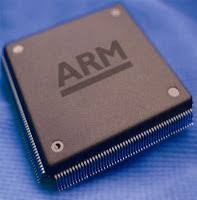
\includegraphics[width=1\textwidth]{figures/ARM.JPG}}
\caption{ARM}
\label{ARM}
\end{figure}

\ref{Cyrix}
\begin{figure}[ht]
\centerline{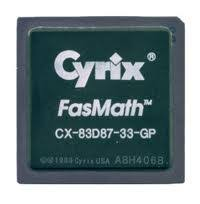
\includegraphics[width=1\textwidth]{figures/Cyrix.JPG}}
\caption{Cyrix}
\label{Cyrix}
\end{figure}

\ref{i5}
\begin{figure}[ht]
\centerline{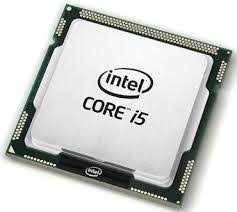
\includegraphics[width=1\textwidth]{figures/i5.JPG}}
\caption{i5}
\label{i5}
\end{figure}

\ref{IntelPentium}
\begin{figure}[ht]
\centerline{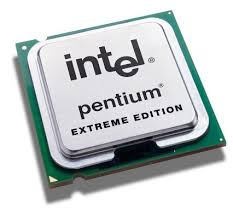
\includegraphics[width=1\textwidth]{figures/IntelPentium.JPG}}
\caption{IntelPentium}
\label{IntelPentium}
\end{figure}

\subsection{Komponen Prosesor}
Prosesor adalah komponen yang terpenting dari sistem komputer, ia juga merupkan pengolah data berdasarkan instruksi yang diberikan kepada
prosesor tersebut,dalam mewujudkan fungsi dan tugasnya prosesor tersusun atas beberapa komponen sebagai anggota dari setuktur CPU, yaitu

\begin{itemize}
	\item Arithmatic dan Logic Unit
	Bertugas untuk membentuk fungsi-fungsi pengolhan data komputer, Arithmatic dan Logic Unit sering disebut sebagai Machine Language
	(mesin bahasa) karena bagian ini mengerjakan instruksi bahasa mesin yang diberikan kepadanya. Arithmatic dan Logic Unit terdiri
	dari dua bagian, yaitu Unit Arithmatika dan Unit Logika Boolean.
	\item Control Unit
	Control Unit bertugas mengontrol operasi CPU dan mengontrol secara keseluruhan komputer, sehingga terjadi sinkronisasi antar komponen
	dalam menjalankan setiap fungsi operasinya.
	\item Register
	Register adalah media penyimpanan internal CPU yang digunakan dalam proses mengolahan data. Memori ini sifatnya sementara biasanya
	digunakan untuk menyimpan data saat dilakukan pengolahan data.
	\item CPU Inter Connections
	Merupakan sistem koneksi dan bus yang menghubungkan komponen internal CPU.
\end{itemize}

\subsection{Perawatan yang Baik Sesuai Prosedur Pabrik}
Hardware atau perangkat keras pada laptop atau komputer merupakan bagian vital yang amat perlu dirawat. 
Seperti halnya prosesor, hard disk, keyboard, layar monitor, baterai, dan sebagainya. 
Semua itu adalah bagian-bagian penting dari komputer yang perlu di perhatikan dan dirawat secara rutin, misalnya
diharapkan agar selalu tidak lupa untuk mengolesi pasta pada bagian atas processor lebih kurang setiap 3 bulan sekali,
casing pc yang memiliki jalur sirkulasi udaranya karena apabila casing tidak memiliki jalur sirkulasi maka komponen yang 
ada didalam pc anda akan lebih cepat panas termasuk pada processor. 


\subsubsection{Perawatan Hardware Secara Umum}

\begin{itemize}	
	\item Jika kita menggunakan laptop dalam waktu yang lama, minimal lima jam sehari disarankan memakai pendingin tambahan dibawah 
laptop anda, yang sering disebut dengan coling pad. Contohnya seperti fan pada laptop. Pendingin ini juaga dapat mengurangi panas 
yang ditimbulkan oleh prosesor, VGA card, dan chipset pada laptop anda.
	\item Selalu bersihkan laptop anda dari debu, terutama pada bagian layarnya dengan menggunakan pembersih laptop atau bisa juga
menggunakan minyak kayu putih. Pada saat membersihkan layar laptop pastikan laptop dalam keadaan mati.
	\item seperti halnya layar pada laptop, keyboard pada laptop juga harus dibersihkan dari debu di sela-sela keyboard secara 
perlahan-lahan.
	\item menggunakan tas khusus laptop yang ada busanya agar ketika laptop dibawa kemana-mana tidak mengalami benturan yang bisa
membuat laptop rusak.
	\item Jangan memberi beban diatas layar, yang nanti akan membuar layar bergaris.
	\item Jangan terlalu sering mereset laptop atau mematikan secara langsung.
	\item Usahakan laptop anda menggunakan penyimpanan listrik sementara, agar ketika saat terjadinya naik turun tegangan tidak
langsung merusak bagian power supply rusak.
	\item Biasakan seminggu sekali untuk scandisk untuk membperbaiki sekto-sektor yang ada di hardisk
	\item Gunakan antivirus agar virus tidak dapat merusak komponen laptop.
	\item Sebisa mungkin diharapkan untuk membersihkan perangkat hardware dalam jangka waktu setiap tiga bulan, menggunakan kuas atau
alat penyedit debu apabila laptop kotor dapat menyebabkan laptop menjadi lamban. Karena antar komponen tidak berjalan dengan
baik.
\end{itemize}

\subsubsection{Cara Merawat Baterai Agar Tetap Awet}
	\subsubsection{Pengisian Baterai atau yang Sering Dikenal Sebagai CHARGING}
	\begin{itemize}
		\item Mengisi baterai sampai penuh pada saat pertama kali membeli laptop.
		\item Ketika baterai kosong, indikator LED akan menunjukkan blink merah, lalu hubungkan AC adaptor untuk mengisi
		baterai.
		\item Pada saat baterai sudah penuh, indikator akan bewarna hijau.
		\item Jangan mengisi baterai dalam waktu yang lama, akan membuat baterai secara perlahan-lahan tidak bisa diisi kembali.
	\end{itemize}
	\subsubsection{Penggunaan Baterai Secara Optimum}
	\begin{itemize}	
		\item Matikan laptop anda jika tidak digunakan.
		\item Tutup LCD jika tidak menggunakan keyboard.
		\item Kontrol pencahayaan LCD untuk menghemat energi.
	\end{itemize}	
	\subsubsection{Pembersihan Pada Baterai Terminal}
	\begin{itemize}	
		\item Lepaskan baterai pada saat laptop tidak digunakan.
		\item Hati-hati cara melepaskannya karena akan menyababkan kontak listrik.
		\item Bersihkan terminal positif dan negatif dengan menggunakan dry cloth.
		\item Selalu matikan laptop anda dan lepaskan AC adaptor bila ingin mengeluarkan baterai dari laptop.
	\end{itemize}
	\subsubsection{Jangan membuat baterai terlalu panas bila penggunaannya bersama-sama dengan AC adaptor, karena dapat 
	menyebabkan excess energi yang mengurangi kapasitas pada baterai.}
	\subsubsection{Rekomendasi kondisi operasi ketika diisi dengan AC adaptor pada suhu 10 derajat celcius sampai
	30 derajat celcius, atau 50 derajat celcius sampai 86 derajat celcius.}
	\subsubsection{Baterai yang bagus dapat diisi kembali minimal 500 kali (kurang lebih usianya 1,5 tahun).}
	\subsubsection{Agar beterai pack di laptop anda dapat bertahan lama, langkah sederhana yang dapat anda lakukan adalah jika
	anda menggunakan laptop pada area yang ada supply listriknya, lepas baterai dulu dan gunakan dengan menghubungkan adaptor 
	langsung ke listrik.}
	
\subsection{Kerusakan dan/atau Kesalah yang Sering Terjadi Pada Prosesor}

\subsubsection{Tiba-tiba Mati}
	\subsubsection{Permasalahan}
Apabila komputer anda tiba-tiba mati dengan sendirinya dan kemudian apabila dihidupkan kembali maka komputer akan hidup lagi dan akan
mati kembali, berarti terdapat masalah pada prosesor.
	\subsubsection{Pengidentifikasi}
Diharapkan aga anda segera melakukan pemeriksaan pada prosesor anda yang terdapat pada perangkat inti atau motherboard, biasanya
masalah yang terjadi yaitu karena prosesor sudah diselimuti oleh debu yang tebal atau bisa juga kipas atau fan procesor tidak
berfungsi secara normal.
	\subsubsection{Solusi}
Solusinya yaitu anda segera membersihkan prosesor komputer anda dari debu dan kemudian, periksa kipas prosesor masih layak pakai
atau tidak, apabila tidak layak pakai diharapkan untuk segera mengganti kipas prosesor anda dengan yang baru.

\subsubsection{Sistem BIOS Tidak Bisa Diakses Saat Booting}
	\subsubsection{Permasalahan}
Apabila komputer atau PC anda tidak mau masuk ke sistem BIOSnya atau tidak mau bekerja secara normal berarti terjadi kesalahan pada
pemasangan prosesor atau prosesor anda sudah habis masa kerja optimal.
	\subsubsection{Pengidentifikasi}
Diharapkan agar anda segera melakukan pengecakan pada prosesor anda, sudah benar atau tidak dalam perletakan prosesor di perangkat
inti. Bisa saja prosesor dipasang secara terbailik atau tidak sesuai dengan arah semestinya yang mengakibatkan prosesor tidak dapat
berfungsi secara normal.
	\subsubsection{Solusi}
Membenarkan perletakan posisi prosesor pada perangkat inti yang sesuai dengan arahnya, atau lebih jelasnya prosesor tidak boleh
dipasang dengan posisi yang tidak semestinya.

\subsubsection{Overheating atau Panas yang Berlebih}
	\subsubsection{Permasalahan}
Overheating atau PC anda mengalami panas yang berlebihan sehingga perangkat anda tidak dapat berjalan normal.
	\subsubsection{Pengidentifikasi}
Melakukan pengecekan trutama pada kipas prosesor terlebih dahulu, apakah kipas prosesor masih berfungsi normal atau tidak, itu
juga merupakan salah satu penyebab terjadinya overheating. Melihat keadaan prosesor penuh dengan debu atau tidak. Melihat juga
keadaan pasta laptop yang berfungsi untuk mendinginkan prosesor sudah kering atau masih basah.
	\subsubsection{Solusi}
Apabila kipas prosesor mati atau tidak terdengar bunyi yang lembut, maka kipas prosesor tersebut harus segera diganti. Apabila
prosesor berdebu maka harus segera dibersihkan dengan cara melepaskan prosesor terlebih dahulu dari perangkat inti, dan
selanjutnya dibersihkan. Mengurangi pemakain PC atau Laptop secara berlebihan, karena dapat mengakibatkan prosesor menjadi
overheating dan otomatis PC atau Laptop anda juga overheating. Mengoleskan pasta yang lebih cair pada prosesor untuk 
menggantikan pasta yang sudah terlanjur kering.

\subsection{Arsitektur Von Neumann}
Kerangka untuk semua komputer modern adalah arsitektur Von Neumann seperti pada gambar \ref{vonneumann}, yang dirinci dalam makalah tahun 1945 oleh matematikawan Hungaria John von Neumann. Ini menggambarkan arsitektur desain untuk komputer digital elektronik dengan subdivisi unit pemrosesan yang terdiri dari unit logika aritmetika dan register prosesor, unit kontrol yang berisi register instruksi dan penghitung program, memori untuk menyimpan data dan instruksi, penyimpanan massa eksternal, dan mekanisme input dan output. 
\centerline{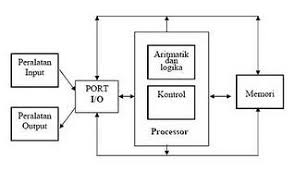
\includegraphics[width=1\textwidth]{figures/vonneumann}}
	\caption{Skema Von Neumann}
	\label{VonNeumann}
	\end{figure}
Arti dari istilah tersebut telah berevolusi untuk berarti komputer program tersimpan dimana pengambilan instruksi dan operasi data tidak dapat terjadi pada saat yang bersamaan karena mereka memiliki bus umum. Ini disebut sebagai bottleneck Von Neumann dan sering membatasi kinerja sistem. \cite{markgrafneumann}

